%!TEX root = ../PhDthesis.tex
\chapter{Exploring the role of inhibition in cortical development}

In the previous chapter we explored the spatially calibrated SCAL
model, establishing how various sources of evidence about the spatial
structure of V1 projections relate to each other. While this model was
able to account for the size-tuning properties of the visual cortex
quite well, it also exhibited two major shortcomings. Most importantly
it highlighted that a model lacking distinct excitatory and inhibitory
populations will not be able to capture the diversity in connectivity
and response profiles that are observed in the mammalian
cortex. Secondly we showed that based on the known lack of truly
long-range inhibitory projections, long-range orientation specific
suppression must be mediated by a di-synaptic mechanism mediated by
long-range excitatory connectivity.

Additionally, in the literature section we described the known
properties of various inhibitory cell classes and what roles they
might perform. In particular we discovered that PV and SOM-expressing
interneurons exhibit highly distinct response properties and
layer-specific expression patterns. With recent techniques enabling
the targeting of specific neural populations, there is now huge
interest in understanding their role both in development and in
mediating and gating both contextual and attentional modulation
phenomena.

In this chapter we will propose a model that incorporate the distinct
response properties of an excitatory pyramidal cell population and the
Parvalbumin expressing interneuron population, allowing us to make
concrete predictions about their role in development. We will
establish that the fast and linear response of the PV-ir, fast-spiking
interneuron population makes them ideally suited towards controlling
feedforward activity, sparsifying activity and thereby driving map
formation. Additionally we will show that this model exhibits more
robust and stable map formation even in the presence of strong lateral
excitation than the previous model.

Specifically we will assess how the model performs when manipulating
the response properties of the PV population, under varying levels of
contrast and strong lateral excitation.

\section{Methods}

\subsection{The SEPI Model}

The \textbf{S}hort-\textbf{R}ange \textbf{E}xcitation \textbf{P}V
\textbf{Inhibition} (SEPI) model is based on the same principles,
spatial profiles and equations that were described for the SCAL model
in the previous chapter. However unlike SCAL the model has a distinct
excitatory and inhibitory V1 population, which both receive afferent
input and are connected to each other recurrently. The architecture
diagram in \ref{SEPIDiagram} shows the two sheets and projections
between them. When comparing this against the SCAL model diagram (see
\ref{SCALDiagram}), we can see that the spatial scales of the various
projections are unchanged they have simply been split up between the
populations.

\begin{figure}
	\centering
        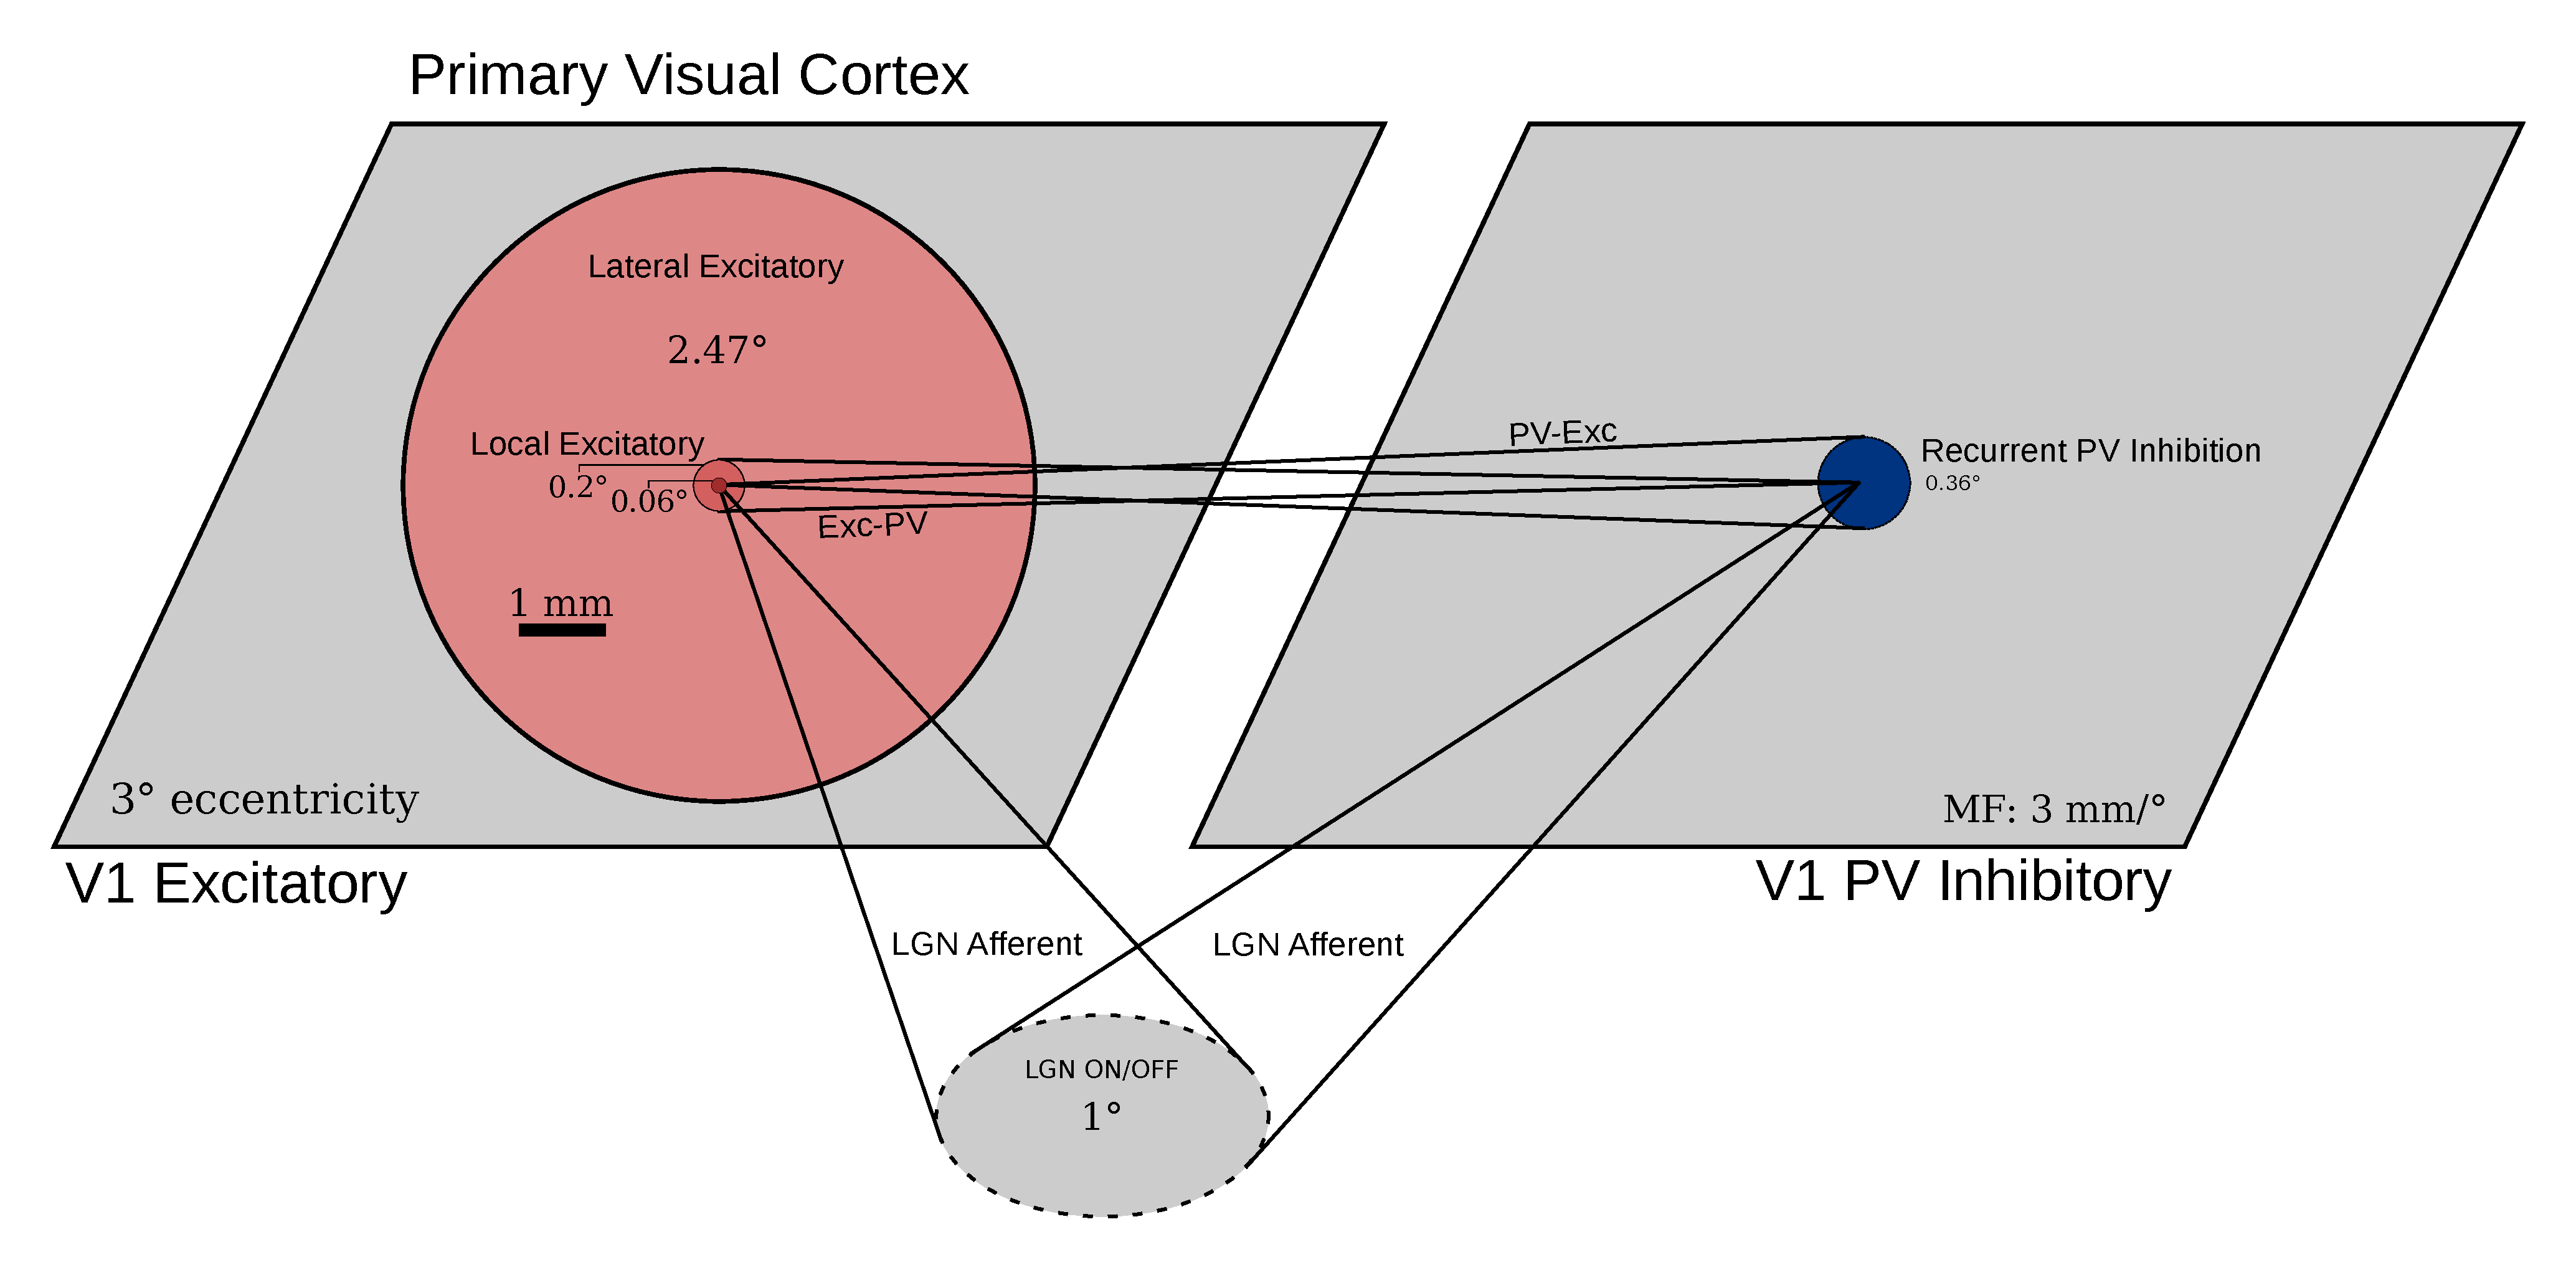
\includegraphics[width=1.0\textwidth]{SEPI_Diagram.pdf}
	\caption{Diagram of the SEPI V1 stage of the model showing the
          spatial scales of the various excitatory (red) and
          inhibitory (blue) connections. Satured colors indicate the
          kernel radii, while lightly shaded regions indicate kernel
          cut-off extents.}
	\label{SEPIDiagram}
\end{figure}

In the literature review we identified the parvalbumin (PV) expressing
interneurons, which include fast-spiking basket and clutch cells, as
the most likely candidate to provide feedforward inhibition and
controlling the gain of the response in of the pyramidal cells. Their
high abundance in the thalamocortical recipient layer 4 and layers 2/3
making up over half the population in each \citep{VanBrederode1990} as
well as their involvement in the onset of critical period
\citep{Fagiolini2000} and effect on the columnar organization of the
visual cortex \citep{Hensch2004} makes them of particular interest. The
other defining characteristics of the PV population is their fast
response \citep{Cruikshank2007,Gabernet2005}, and their ability to
linearly match the excitation in the excitatory population
\citep{Atallah2012}. This closes matches the role of the inhibitory
projection in the SCAL model, which provides divisive gain control and
is directly coupled to the response of the excitatory population.

The equations governing the responses of both the excitatory and
inhibitory population are also unchanged, driven by summing the
excitatory input and divided by the inhibitory activity. This closely
matches what we know about PV neurons in the cortex, which provide
strong peri-somatic synaptic inputs to spiny neurons, providing
shunting inhibition \citep{Atallah2012, Wilson2012}. Based on tracing
studies we know that excitatory and inhibitory neurons and
specifically the Parvalbumin expressing subpopulation strongly and
densely innervate each other and themselves \citep{Buzas2001, Ma2011,
  Pfeffer2013}. Additionally these PV population receive strong
afferent input \citep{Burkhalter2008}. All three of these properties
are captured directly by the model.

In order to capture the response of the PV population we apply only
half-rectification to the inhibitory population, as basket cells
generally have a very low spiking threshold \citep{Ma2011}, and the
difficulty involved in balancing homeostatic thresholds in two
populations. Secondly we keep the effect of the inhibition divisive in
their effect on both each other and on pyramidal cells. These
properties distinguish them from the other major class of inhibitory
interneurons the somatostatin (Sst) expressing population, which
receive weaker but facilitating inputs
\citep{Beierlein2003,Bartley2008,Tan2008}.

\subsubsection{Activation}

The activation for both the excitatory and inhibitory population is
given by:

\begin{equation}
  \eta_{exc/inh} = \frac{\eta_{A} + \eta_{Loc-Exc}}{1 + \eta_{PV-Inh}}
\end{equation}

where $\eta_{A}$ is the LGN afferent activity, $\eta_{Loc-Exc}$ the
local excitatory contribution and $\eta_{PV-Inh}$ the PV inhibitory
contribution. In other words both population integrate over afferent
and local excitatory input and are then divisively normalized by the
PV population. Optionally an additional long-range excitation term can
be added to modulate the activity dependent on long-range excitatory
input:

\begin{equation}
  \eta_{exc} = \frac{\eta_{A} + \eta_{Loc-Exc}}{1 + \eta_{PV-Inh}} (1+\eta_{Lat-Exc})
\end{equation}

where $\eta_{Lat-Exc}$ is the input from the lateral excitatory
projection.

\subsubsection{Hysteresis}

In order to control the temporal properties of the PV population we
introduce a hysteresis term, which is disabled in the final
model. This will allow us to test the importance of fast inhibition in
the model. The hysteresis function is defined as a discrete
exponential weighting between the previous activation and the new
activity, expressed as:

\begin{equation}
  \eta_h (t + \delta\eta) = \eta(t) + \tau \big[ \eta(t+\delta\eta - \eta(t) \big]
\end{equation}

where $\tau$ is the time constant. This will effectively slow down PV
responses relative to the excitatory population. In the final model
this term is eliminated simply by setting $\tau = 1$.

\subsection{Assessing the quality of orientation maps} \label{metrics}

A major component of the analysis applied in this section is to assess
the sensitivity of the model to changes in the response properties of
the different cell classes. Therefore we have to establish a number
metrics to assess the robustness of the model to changes in contrast
by assessing the quality of orientation map organization of the
excitatory V1 neurons map. There are a variety of measures to assess
these properties but we will focus on three in particular, smoothness,
stability and pinwheel density.

\subsubsection{Pinwheel density}

Through empirical observation that orientation maps across species
share a fundamental property, that pinwheel count in biological
orientation maps scales linearly with hypercolumn size, specifically
that there are $\pi$ orientation pinwheels within the area of one
hypercolumn, when averaging over sufficiently large cortical
areas. This dimensionless, statistical measure of pinwheel
distribution is thought to reflect a universal constant of map
organization, converging to across carnivorans, primates, cats, and
tree shrews \citep{Kaschube2010, Keil2012}. This value was predicted
by a theoretical model of map organization and has strong empirical
evidence, with a mean pinwheel density across four species (tree
shrew, galago, cat, and ferret) statistically indistinguishable from
$\pi$.

To determine the pinwheel density for any given map, the hypercolumn
distance is computed and all all pinwheel centers are found. Pinwheel
centers are located at the intersection of the zero contours of the
real and imaginary components in the polar representation of
orientation preference \citep{Lowel1998}. Then we simply divide the
number of pinwheels in the modeled area by the number of hypercolumns
to arrive at the pinwheel density.

\subsubsection{Orientation Selectivity}

When measuring an orientation map using the protocol outlined in
\ref{ORMeasurement} two components are returned, the first is the
orientation preference, which corresponds to the orientation at which
there was a maximal response. Additionally there is a selectivity
components, which provides a measure of how much the neuron responded
to the preferred orientation relative to all other orientations. This
provides a simple metric to assess how selective a neuron is and can
easily be averaged across all neurons in a central region to get an
average selectivity value.

\subsubsection{Stability}

The stability of orientation maps is determined by determining the
average orientation similarity index of the orientation map over the
course of development. To assess similarity quantitatively,
\cite{Chapman1996} computed the difference of orientation preference
at each developmental age with the organized preference map observed
in the final recording for that animal. As in \cite{Stevens2013} we
normalize these similarity values to fall between 0 (completely
uncorrelated) to 1 (identical orientation preference). The orientation
similarity index is therefore defined as:

\begin{equation}
  OSI = 1 - \frac{4}{n\pi} \sum_{i}\abs{(F_{i}-O_{i})mod(\frac{\pi}{2})}
\end{equation}

By averaging the OSI at every 1000 development steps we can
numerically compare the stability of the model over time. Note that
this does not provide a measure that is comparable across models
because this measure is heavily influenced by the speed of learning
but it does allow us to assess the effect of changing specific
parameters on the stability of the model.

\subsubsection{Local Homogeneity Index}

The local homogeneity index (LHI) was first introduced by
\cite{Nauhaus2008} as measure of the local smoothness of the map. It
is therefore useful to determine whether a neuron is in a smooth
region of the orientation map or near a pinwheel region where the
orientation preference varies considerable. The LHI is defined based
on a specific $\sigma$ value, which should reflect the spatial
properties of the map. Therefore we can use the mean LHI across the
entire map as a measure of the scale of homogeneous regions of the
map. The LHI at location x is computed as follows:

\begin{equation}
  LHI(x) = \frac{1}{2\pi \sigma^2} \bigg\lvert \int
  exp\bigg(\frac{-\|x-y\|^2}{2\sigma^2}\bigg) exp(i2\theta_y) dy
  \bigg\rvert
\end{equation}

where, $\theta_y$ is the orientation preference at site y and $\sigma$
determines the spatial scale of the analysis. In their experiments
\cite{Nauhaus2008} used $\sigma=180\mu m$ to match the spatial extent
of dendritic fields in both cat and monkey cortex.

\subsubsection{Center-of-Gravity Distortion}

Since we have access to all the weights in the model we can compute
the center-of-gravity (CoG) of the afferent weights relative to
position of the neuron, to determine how much distortion to the
retinotopy each neuron exhibits. The CoG along one axis is computed as
the mean of normalized vector product:

\begin{equation}
  CoG(p, \omega) = \frac{1}{\sum_i \sum_j \omega_{i, j}} \sum_i \sum_j \omega_{i,j} p_{i,j}  
\end{equation}

where $p$ is the position along either the x- or y-axis and $\omega$
is the weight at that location. The distortion in the CoG is then
given by euclidean distance between the center of gravity and the
actual location of the neuron:

\begin{equation}
  CoGD(x, y) = \sqrt{(CoG_x-x)^2 + (CoG_y-y)^2}
\end{equation}

By computing the shift for all neurons in a central regions we can use
this metric as a measure of the quality of the retinotopic mapping in
the model, highlighting significant distortions introduced by
unbalanced excitation and inhibition.

\section{Results}

\subsection{Development}

The role of inhibition in development is hugely important, as
evidenced by the fact that a variety of pathological conditions
including autism \citep{Wohr2015} and schizophrenia \citep{Lewis2012}
have been tied to changes in PV-expressing interneurons in the
cortex. Modeling the role of these cell classes in development and
specifically a rate-based modeling requires capturing their response
properties. Since the synaptic projection develop as a result of these
properties, the tuning properties of the modeled neurons in the
developed model will let us concrete predictions about the role of
these neurons in shaping the development.

Accurately capturing the response of these neurons in a rate-based
model presents a number of challenges. Additionally a lot of the data
about these cell classes comes from mouse data where the genetic
manipulation of specific cell classes has recently become possible. At
the same time this provides a great opportunity to establish whether
the coarse response properties of the neurons can predict their final
tuning properties in the model and how manipulating them can affect
both development and the instantaneous response of the model to
specific stimuli.

In spatially calibrating the connections between neurons in the SCAL
model we had already focused on the PV population, so calibrating the
inputs and response properties of these neurons is the next step. The
literature is very clear that PV neurons in the visual cortex receive
strong inputs both from thalamocortical afferents and from recurrent
inputs, so the main question to settle is how closely these neurons
are coupled to the excitatory population. If the hypothesis that these
neurons can quickly and robustly balance out the excitation arriving
from the LGN \citep{Swadlow2003, Burkhalter2008}, by linearly matching
the response of the pyramidal cell population and providing contrast
gain control to sparsify the activity and thereby sharpen the
orientation tuning \citep{Wilson2012}, then a non-linear and very slow
response among this population should disrupt map development.

\subsubsection{Linearity and time profile of inhibitory responses}

In order to explore these effects the model was launched with varying
activation functions. The first component would vary the linearity of
the response by adding an exponential term after the
half-rectifier. By varying this exponential term we could vary the
response of the neuron from between sub- and supra-linear
values. Additionally a hysteresis term was added to control the time
profile of the response. After training the models were then assessed
based on the metrics outlined in \ref{metrics}.

The results of the parameter exploration are shown in figure
\ref{SEPILinearity}. They include a measure of stability over time,
orientation selectivity, distortion of the retinotopy, the mean local
homogeneity index (LHI) and finally the pinwheel density ($\rho$),
used to assess the quality of the maps.

The immediately striking result is that narrow band of good (near
$\pi$) pinwheel densities in the linear region of the response. Apart
from that we can clearly see that orientation selectivity, stability
and the CoG distortion are strongly correlated, while they are
anti-correlated with the LHI. In particular, we can see increasing
distortion of the retinotopy as the inhibitory population responds
more strongly, which causes serious disruptions to the map quality. At
the same time sub-linear responses seem to induce very weak
selectivity, which causes relatively low stability and high
homogeneity.

\begin{figure}
	\centering
        \includegraphics[width=1.0\textwidth]{./results/sepi/SEPI_Linearity.pdf}
	\caption{Parameter exploration to determine how the linearity and
      time constant of inhibitory responses affect development. A) A
      measure of stability of the model over time, integrating the
      similarity index of the model over time. B) Orientation
      selectivity in the model measured using orientation map
      measurements. C) The average local homogeneity index measuring
      the smoothness of the map at a particular spatial scale. D)
      Pinwheel density of the model, which should approach $\pi$ for a
      perfect map. E) The Center-of-gravity (CoG) distortion provides
      a measure of how much the retinotopy in the model has been
      disrupted.}
	\label{SEPILinearity}
\end{figure}

In order to get a better overview of the relationships between these
variables The correlation matrix between the independent variables
we're exploring and the metrics can be seen in
\ref{SEPILinearityCorr}. This highlights once again the strong
relationship between orientation selectivity, stability and the CoG
shift and supra-linear PV cell responses. This view makes it clear
that the PV cell exponent has a much greater effect on the various
metrics than the time constant of the response, which does not show
significant effects until the response is very slow.

\begin{figure}
	\centering
        \includegraphics[width=0.7\textwidth]{./results/sepi/SEPI_Linearity_Correlations.pdf}
	\caption{A correlation matrix of the various dependent and
      independent variables of the linearity analysis. Plots the
      Pearson correlation of the various metrics against each other.}
	\label{SEPILinearityCorr}
\end{figure}

Overall we can conclude that a linear response but not necessarily a
very fast response is required to drive the development of a
high-quality orientation map. We will attempt to disentangle the
causal relationships between these variables in the
discussion. However we now have a strong claim that we can develop
high-quality orientation maps in the model. As a next step we will
investigate how this model compares to the SCAL model.

\section{The SEPI Model}

The idea behind developing a model with distinct excitatory and
inhibitory populations was based on three main observations. The first
is straightforward, we know that in biology a single class of neurons
will never provide both excitation and inhibition, also known as
Dale's law. From this perspective the SEPI model already provides an
advantage over the SCAL model. However we also wanted to see whether
this model could improve the diversity in responses and more
accurately capture contrast-dependent responses in the model, while
continuing to develop high quality maps and exhibiting robust and
stable self-organization.

The linearity analysis already confirmed the model could produce
high-quality orientation maps. In \ref{SEPIORTuning} this is further
confirmed with a high-quality map, and clearly defined receptive
fields, which exhibit contrast invariant orientation tuning, which
rivals previous models. Without going into two much more detail, we
could also confirm that the spatial calibration still holds,
exhibiting ~3.5 cycles per visual degree, well within the acceptable
margins that were established in \ref{SCALHypercolumns}.

\begin{figure}
	\centering
    \includegraphics[width=1.0\textwidth]{./results/sepi/SEPI_V1_ORTuning.pdf}
	\caption{SEPI model orientation tuning properties after presenting
      20,000 oriented Gaussian patterns. A) Orientation map measured
      by presenting sine gratings at the optimal spatial frequency to
      the model, along with the locations of the receptive fields
      shown in B. B) Gabor-fits to receptive fields measured using
      sparse random noise. C) Orientation tuning curve of a single
      neuron across contrasts, demonstrating largely
      contrast-independent orientation tuning.}
	\label{SEPIORTuning}
\end{figure}

The main thing we are interested in however is how decoupling the two
populations affects contrast-dependent size-tuning shifts, which rely
on strong divisive inhibition. Recall for example that the GCAL model
showed very little contrast-dependent size-tuning changes due to the
inhibition being purely subtractive. The SCAL model demonstrated a
strong shift, however it severely lacked in diversity. Repeating this
same protocol in the SEPI model as is shown in
\ref{SEPI_DoG_Contrast}, demonstrates a slightly larger shift in
contrast-dependent size tuning, that is in fact exactly in line with
other measurements performed in macaque (~2.2x). However more
strikingly the model now exhibits a large degree of diversity in size
tuning shifts, which provides a much better match to experimental
results (see \ref{ContrastShift}).

\begin{figure}
	\centering
        \includegraphics[width=0.8\textwidth]{./results/sepi/SEPI_V1_DoG_Contrast.pdf}
	\caption{contrast-dependent shifts in size tuning as estimated by
      the DoG model. A) Spatial constant of the excitatory center of
      the DoG model at low vs. high contrast. B) Distribution of
      contrast-dependent shifts, showing a much better match to the
      experimental data than GCAL or SCAL (see \ref{ContrastShift}).}
	\label{SEPI_DoG_Contrast}
\end{figure}

Introducing a separate inhibitory population also allows us to compare
the spatial and orientation profile of inhibitory neurons more
realistically since they no longer reflect the activation of the joint
excitatory/inhibitory population. When comparing
\ref{SEPI_OR_Distributions} we can see that the neurons are no longer
as strongly biased toward the preferred orientation of the excitatory
neuron, this is a direct result of much broader orientation tuning in
the inhibitory PV population.

\begin{figure}
	\centering
        \includegraphics[width=1.0\textwidth]{./results/sepi/SEPI_Inh_OR_Distributions.pdf}
	\caption{Spatial distribution of weights targeting A)
      iso-orientation regions, B) oblique-orientation regions and C)
      cross-orientation regions.}
	\label{SEPI_OR_Distributions}
\end{figure}

Finally we can confirm the spatial and orientation tuning properties
of the SEPI model in another way. By computing the local homogeneity
index as we did above, we can compute the smoothness of the map at a
specific spatial scale. Since we know the spatial scales in the model
we can directly compare the distribution of the LHI to experimental
data. The $\sigma$ value was therefore set to $180 \mu m$ and plotted
against the orientation tuning width of all neurons in a central
region of the simulated map. The resulting scatter plot is shown in
\ref{SEPILHI}, compared directly to equivalent measurements in macaque
and cat visual cortex. Both the distribution of tuning widths and LHI
values match the experimental data from macaque, but not cat, very
well, which is exactly what was desired.

\begin{figure}
	\centering
        \includegraphics[width=0.6\textwidth]{./results/sepi/SEPI_LHI.pdf}
	\caption{Local homogeneity index against tuning width in the SEPI
      model compared to experimental results from monkey and
      macaque. Reproduced from \cite{Nauhaus2008}.}
	\label{SEPILHI}
\end{figure}

While the model now exhibits many of the properties that were lacking
in the SCAL model one last issue remains. A large reason why the SEPI
model was introduced in the first place was to come up with a model
that would exhibit realistic long-range connectivity, which is
presumed to underly various contextual modulation effects. In this
next section the effect of introducing long-range excitatory on the
development of the model will be explored to see whether this model
can robustly develop even in the presence of the long-range patchy
connections that are so characteristic of pyramidal cells in layer 2/3
of the cortex.

\subsubsection{Robustness to long-range excitation}

At this point two separate models have been introduced, the SCAL and
SEPI models, which are very similar differing mostly by the fact that
the latter has distinct excitatory and inhibitory populations. The
major reason why the populations were split in this way is to match
the anatomy, but does this actually buy us anything from a functional
perspective? In order for long-range excitation to mediate contextual
modulation phenomena, these projections need to be able to
meaningfully modulate neuron activity at long distances. However from
a theoretical perspective introducing strong long-range excitatory
connectivity in a model seems problematic for a number of
reasons. Ignoring the fact that strong excitation can lead to runaway,
`epileptic` activity in the cortex. More subtly however, by
introducing long-range correlations into the activity we can disrupt
the retinotopy in the model and violate the sparse coding hypothesis,
which have been shown to play crucial roles in self-organization.

Therefore assessing how the models hold up in the presence of strong
lateral excitation under varying contrast levels will help us
establish how robust the model is and lay the groundwork for a model
that exhibits both long-range excitation and suppression. Therefore we
will compare how the SCAL and SEPI models deal with varying levels of
contrast and lateral excitation to investigate whether separating the
populations has any benefits in addition to being more anatomically
realistic.

The results of this analysis once again assessed by the list of
metrics described above is shown in \ref{SCALStability}. The first
thing to note is that increasing lateral excitation leads to immediate
disruptions to the self-organization of the model until we reach a
transition point at which the model fails to self-organize completely,
presumably this is where the additional excitation can no longer be
balanced by increases in the gain of inhibition. Indeed the CoG
distortion increases with increasing lateral excitation suggesting
that activity is allowed to propagate from where it arrives in V1
leading to disruptions in retinotopy. In summary we can see that
strong lateral excitation causes disruptions to the stability,
orientation selectivity, pinwheel density and CoG distortion causing
the eventual breakage of the entire model.

\begin{figure}
	\centering
        \includegraphics[width=1.0\textwidth]{./results/SCAL/SCAL_Robustness.pdf}
	\caption{Parameter explorations of three separate metrics of
          orientation map development using the SCAL model. Varied
          parameters are the strength of long-range lateral excitation
          and the stimulus contrast. The three metrics are \textbf{A}
          the $\rho$ pinwheel density metric, which characterizes the
          quality of the map, \textbf{B} the average selectivity over
          the time course of development and \textbf{C} the stability
          metric measuring how much the map changes throughout the
          course of development. The model shows good robustness to
          varying stimulus contrasts at low levels of lateral
          excitation but quickly deteriorates with increasing levels
          of excitation. White values indicate instabilities in the
          model causing the model to terminate.}
	\label{SCALStability}
\end{figure}

The correlation matrix, shown in \ref{SCALRobustnessCorr} highlights
what is going wrong as we increase the lateral excitation. It
demonstrates a strong relation to CoG distortion and increasing
homogeneity, with clear anti-correlation with orientation selectivity
and stability. As a result we can conclude that the lateral excitation
leads to disruptions in retinotopy and lower selectivity, which in
turn disrupt the stability and pinwheel density of the model.

\begin{figure}
	\centering
       \includegraphics[width=1.0\textwidth]{./results/SCAL/SCAL_Robustness_Correlations.pdf}
	\caption{A correlation matrix of the various dependent and
      independent variables of the linearity analysis. Plots the
      Pearson correlation of each variable against each other
      variable.}
	\label{SCALRobustnessCorr}
\end{figure}

When applying the same analysis to the SEPI model strikingly we can
see that the model shows very little disruptions at equivalent levels
of lateral excitation. As can be seen in \ref{SEPIStability}, the
model shows basically no CoG distortion, and very little variation in
pinwheel density, stability and LHI. The orientation selectivity on
the other hand actually increases with both excitation and contrast,
the opposite to what was observed in SCAL. However even this model
begins to break down under very high contrast and strong lateral
excitation.

\begin{figure}
	\centering
        \includegraphics[width=1.0\textwidth]{./results/sepi/SEPI_Robustness.pdf}
	\caption{Parameter explorations of three separate metrics of
          orientation map development using the SEPI model. In
          comparison to the SCAL model the pinwheel metric is not as
          robust to changes in contrast, however the model is far more
          robust to strong lateral excitation and maintains almost
          uniform stability across almost all explored parameter
          values. Uncoupling of excitation and inhibition allows the
          model to handle changes in parameter strengths but in
          absence of a homeostatic mechanism may disrupt map formation
          at low contrasts.}
	\label{SEPIStability}
\end{figure}

Overall however the SEPI model is significantly more robust to
variations in the strength of afferent input and even lateral
excitation, which is usually thought to cause problems for models,
which rely on competition between neurons to represent the visual
space.

\section{Discussion}

In this chapter we have explored how distinct excitatory and
inhibitory modeled after the pyramidal and basket cells in the visual
cortex interact to give rise to robust and stable map formation and
then confirmed the model still matches the other spatial and
orientation tuning properties we carefully evaluated in the SCAL
model.

\subsection{The role of inhibition in development}

In the first experiment we asked what happens when we decouple the
responses of the inhibitory population from that of the excitatory
population. In the SCAL model and all most previous SOM based models
both excitatory and inhibitory cells were represented by the same
neurons, which means their responses were coupled directly. While the
time constant had very little effect on the organization of the model
the analysis highlighted how strong an effect a non-linearity in the
activation function of the inhibitory population had. A sublinear
response was associated lower selectivity, stability, while a
supra-linear response was associated with very high orientation
selectivity but also greater distortion in the retinotopy.

From a theoretical perspective this makes sense, the PV population is
able to match the level of excitation that is arriving in the cortex
from thalamocortical afferents and recurrent intra-cortical
connections and shifting that balance in either direction will disrupt
the development. Indeed if we compare the effect of upregulating the
PV responses we can see some parallels to what happens during
pharmacological upregulation of $GABA_A$ neurons by administering the
$GABA_A$ agonist benzodiazepine (diazepam)
\citep{Fagiolini2004,Hensch2004}, which looked at ocular dominance
columns rather than orientation columns. Much like in those
experiments the neurons become more segregated and selective when the
inhibitory population was upregulated in this way. At the same time
however the column size actually narrowed, which is the opposite
effect to what was observed in those experiments.

Finally we compared how the SCAL model compared to the SEPI model in
terms of robustness to lateral excitation and varying levels of
contrast. These results clearly showed that the SEPI model
self-organizes across for a wider range of lateral excitation values
indicating it can deal with the potential disruptions caused by
introducing long-range excitation much better. This is likely a direct
result of separating the two populations. Although this allows these
neurons to become uncoupled it also ensures that the inhibitory
population can effectively respond and cancel out the additional
excitation arriving via long-range connections. However at the highest
lateral excitation and contrast values tested here even this model had
trouble canceling out this additional excitation. It is also worth
noting these models were both trained on simple Gaussian patterns,
which exhibit no long-range correlations, which might disrupt the map.

Based on these observations it seems that the PV population at least
in the model provides a means for neurons to compete in a local region
to represent the stimulus and repelling neurons with similar feature
preferences which results in a smooth local mapping of the stimulus
features into an orientation map. Since the neurons respond so quickly
and robustly this ensures the development of a good orientation map
even in the presence of other influences, but also means that
pathological changes in the PV response properties could severely
disrupt the organization of the cortex.

\subsection{Feature tuning and Inhibition}

In analyzing the model size and contrast response we showed very good
agreement with experiment and indeed the variability in responses was
greatly improved over what was observed in the SCAL model. By
decoupling the excitatory and inhibitory neurons we showed we could
achieve a greater contrast-dependent size-tuning shift both
qualitatively and and quantitatively much closer to the kinds of
shifts that are seen in experiment (see \ref{SEPI_DoG_Contrast} and
\ref{ContrastShift}). This agree very well with the idea that the PV
neurons exert strong control over the response gain of principal
neurons via a divisive mechanism \citep{Wilson2012}. Indeed through
artificial upregulation of the PV population we could mirror the
effects of decreasing the contrast, a result that was first confirmed
by \cite{Nienborg2013} in mouse visual cortex.

One major question in the literature surrounded the question of the
tuning properties of PV neurons. A number of theoretical studies had
suggested that untuned or broadly tuned inhibition in the visual
cortex was required for the development of orientation selectivity or
its contrast invariance \citep{Somers1995, Troyer1998}. The work by
\cite{Cardin2007} challenged this assumption as they had found that
the fast-spiking cells in layer 4 of cat area 17 did not exhibit
significantly broader tuning than the regular spiking excitatory
population. However, they did find broader tuning in the spiking
response in this population and similar studies had found conflicting
results \citep{Hirsch2003, Nowak2008}. In the SEPI model the cells
generally display orientation tuning, however they are overall
significantly more broadly tuned than the excitatory population, this
is largely driven by the fact that the modeled cells do not have any
spiking threshold. \cite{Cardin2007} argue studies such as
\cite{Nelson1994}, which demonstrated no widening in orientation
tuning of excitatory cells under GABAergic inactivation suggests that
broad inhibitory tuning does not significantly contribute to
sharpening of orientation tuning. However this ignores the role of
inhibitory neurons in shaping the responses and tuning of neurons
during development, such that the instantaneous responses of the
inhibitory population aren't needed to significantly sharpen the
tuning of excitatory cells, as their tuning has already been encoded
in the feedforward connections.

Another difficulty is in determining layer specific effects,
\cite{Cardin2007} primarily measured from fast-spiking cells in layer
4. It may be the case that fast-spiking neurons in layer 4 are more
closely involved in a push-pull inhibitory regime, which would require
sharper orientation tuning \citep{Hirsch2003, Hirsch2006a}. Further
investigation will be required to determine the precise properties of
the PV-ir neuron population across layers in species with maps, in
order to determine whether there are functionally distinct subgroups.

\subsection{Conclusion}

Overall the results here indicate that the PV population is very well
suited towards mediating the kinds of tasks that are important both
for robust development. Specifically they can linearly track the
responses of pyramidal cells in their vicinity by integrating
feedforward and recurrent input and matching the levels of excitation
in these neurons. This leads to a model that is highly robust to
long-range excitation but still exhibits the important properties of
the SCAL model including contrast invariant orientation tuning and the
same spatial tuning. At the same time however the model still has no
way of mediating any true long-range inhibitory effects.

Since the PV population is only weakly tuned for orientation it is not
clear how they could mediate any orientation specific effects such as
iso-orientation suppression, which are well established in the
cortex. Indeed we have not yet established whether long-range
statistical relationships in the visual input would cause significant
disruptions to the self-organization of the model. In the next chapter
we will therefore investigate the interaction between visual
statistics, surround modulatory effects and the effect of both on the
development of the model.
